% !TEX root = thesis.tex
\section{Resources}
\label{sec:resources}

It makes sense at this point (if not earlier), to discuss what language resources are. There are two main types of resources: corpora and tools which act on corpora. They are inextricably linked, but the approaches towards building, archiving, and using either differ. This section seeks to answer one question: what resources are needed to take a language from no resources, to a thriving language with a large digital presence?

For digital vitalisation, \citet{kornai2015new} proposes working on a pyramid approach: first build a corpus with active and engaged speakers, then l10n and i18n support; then word-level tooling such as spell checkers and morphological analysers; phrase and sentence level tooling such as parsers; and finally speech and character recognition and machine translation. This, in general, follows how most language development progresses. However, a finder grained understanding of the tools would be illuminating. While an exposition of all possible natural language processing tools is beyond the scope of this thesis, it is worth going into some depth about some of them.

It is worth noting here that there are different groups which work on each of the stages of language development. Abstractly, these could be defined as language communities and linguists, and the fields of computational linguistics and natural language processing (NLP). The first group are those - often not computational linguists by training or NLP researchers - who want their own language or the language they are studying to exist digitally and in some form. The initial step is generally to adopt any language script, whether pre-existing or ready-made for the language by linguists (for examples of this, see the Endangered Alphabets Project\footnote{\href{http://endangeredalphabets.com/}{http://endangeredalphabets.com/}}) into Unicode, a standard for consistent character representation.\footnote{\href{https://unicode.org/}{https://unicode.org/}} There are linguistic research groups that focus on this problem; for instance, the Script Encoding Initiative at Berkeley.\footnote{\href{http://linguistics.berkeley.edu/sei/index.html}{http://linguistics.berkeley.edu/sei/index.html}}

Some of the people involved in this process may be computational linguists. \citet{bender2016linguistic} makes a distinction between the fields of computational linguistics and NLP: "computational linguistics is used to describe research interested in answering linguistic questions using computational methodology, while natural language processing describes research on automatic processing of human language for practical applications." It should be clear here that computational linguistics is a subfield of linguistics, and that the two are not always in sync, as for instance \citet{kay1997proper} points out when discussing improving machine translation (ML) by using informed linguists. \citet{bender2010grand, bender2016linguistic} goes further, suggesting that understanding language typology can drastically help with multilingual NLP. Many experts in NLP would not consider themselves computational linguists, but developers, just as many language developers would not consider themselves linguists. While navigating the field or looking at resources, it is important to keep these distinctions in mind, as they inform narratives concerning resource generation, scope, and efforts.

\subsection{Resource Aggregators}
\label{subsec:resource-aggregators}

I've already mentioned that Cr\'ubad\'an \citep{scannell2007crubadan} is a good location to find monolingual texts from the web; however, this is but one of an almost infinite amount of corpora that might be of use to linguists, language activists, and to NLP practitioners. To find other resources can be an overwhelming task. To help solve this issue, there are a non-trivial number of large organisations and databases where it is possible to find resources - dictionaries, academic references, and occasionally software - on low resource languages. \citet{unesco11directory} for instance itemises hundreds of such resources. To give more of an idea of what these resources are like, here are some major examples:

\begin{itemize}
\item The Unicode Common Local Data Repository (CLDR) "provides key building blocks for software to support the world's languages, with the largest and most extensive standard repository of locale data available."\footnote{\href{http://cldr.unicode.org/}{http://cldr.unicode.org/}} There are dozens of scripts available in Unicode.\footnote{\href{https://www.unicode.org/standard/supported.html}{https://www.unicode.org/standard/supported.html}}

\item The Endangered Languages Project (ELP), described above and in \citet{lee2016assessing} and online\footnote{\href{http://www.endangeredlanguages.com/}{http://www.endangeredlanguages.com/}} has information on many under resourced languages.

\item Ethnologue, which is both a book \citep{lewis2009ethnologue} and an online resource,\footnote{\href{https://www.ethnologue.com/}{https://www.ethnologue.com/}} is the most comprehensive resource describing the world's languages, such as population size and the general geographic locations of speakers. It is published by SIL International, an evangelical Christian non-profit organisation, and has proprietary paywalls for repeated access to content. Many SIL entries for specific languages include academic references.

\item Glottolog\footnote{\href{http://glottolog.org/}{http://glottolog.org/}} is an open source alternative to Ethnologue, developed at the Max Planck Institute for Evolutionary Anthropology. It has over 180,000 references, with information on over eight thousand languages. \citep{hammarstrom2015glottolog}

\item Omniglot, "the online encyclopaedia of writing systems and languages",\footnote{\href{http://omniglot.com}{http://omniglot.com}}, contains around writing information for around a thousand languages. \citep{ager2008omniglot}

\item The Online Database of Interlinear Text (ODIN)\footnote{\href{http://odin.linguistlist.org}{http://odin.linguistlist.org}} is a multilingual repository of annotated language data for 1274 languages.\footnote{Noted as of January 13, 2010; Accessed April 17, 2018. \href{http://odin.linguistlist.org}{http://odin.linguistlist.org}} The database is formed by crawling scholarly articles on the web and looking for interlinear glossed text (IGT), an industry standard for displaying corpora in academic linguistics by displaying the original datum, a morphosyntactic gloss, and a translation. These data are not massive, but they are useful in particular for training algorithms on structured data. As well, "ODIN was developed as part of the greater effort within the GOLD Community of Practice \citep{farrar2007gold} and the Electronic Metastructure for Endangered Languages Data efforts (EMELD)\footnote{\href{http://emeld.org/}{http://emeld.org/} and \citet{farrar2002common}}, whose goals are to promote best practice standards and software, specifically those that facilitate interoperation over disparate sets of linguistic data." \citep{lewis2010developing}

\item The Open Language Archives Community (OLAC), a worldwide virtual library of language resources \citep{simons2003open}.\footnote{\href{http://www.language-archives.org/}{http://www.language-archives.org/}}

\item Wikipedia,\footnote{\href{https://www.wikipedia.org/}{https://www.wikipedia.org/}} "the largest and most popular general reference work on the Internet" \citep{wiki:Wikipedia} has a nontrivial amount of articles on low-resource languages, many of which have references themselves to Scholarly work. \citet{kornai2013digital}, among others, notes that Wikipedia is one of the first ports-of-call for new language communities, and while it is not a precondition for having corpora on the web, it is a {\it sine qua non} for digital vitalisation. Thus Wikipedia has two purposes; documenting the language and its community (for instance, in the Naskapi Language article\footnote{\href{https://en.wikipedia.org/wiki/Naskapi\_language}{https://en.wikipedia.org/wiki/Naskapi\_language}}), and providing a space for corpus development in the target language itself.

\item The World Atlas of Language Structures (WALS) is a directory typological features which also includes academic references for many of the over two thousand languages presented. WALS is a curated resource, largely made by a team of 55 experts, and hosted by the Max Planck Institute for Evolutionary Anthropology (the same as Glottlog, and as other resources such as PHOIBLE\footnote{\href{http://phoible.org/}{http://phoible.org/}} \citep{phoible} and DOBES\footnote{\href{http://dobes.mpi.nl/}{http://dobes.mpi.nl/}} \citep{wittenburg2003dobes} related to taking an inventory of language structures). \citep{wals}

% are the LREMap ([2], [17]), the CLARIN Virtual Lan- guage Observatory 16, the catalogues of Linguistic Data Consortium17, ELRA18 and META-SHARE19. From soria 2017

%  ELRA, LDC, NICT Universal Catalogue, ACL Data and Code Repository, OLAC, LT World.

\end{itemize}

There are other resources: the CLARIN Virtual Language Observatory\footnote{\href{https://vlo.clarin.eu}{https://vlo.clarin.eu}}, the Linguistic Data Consortium at UPenn,\footnote{\href{https://www.ldc.upenn.edu/}{https://www.ldc.upenn.edu/}} the ELRA,\footnote{\href{http://catalog.elra.info}{http://catalog.elra.info}} META-SHARE,\footnote{\href{http://www.meta-share.eu/}{http://www.meta-share.eu/}} the Association for Computational Linguistics' Wiki,\footnote{\href{https://aclweb.org/aclwiki}{https://aclweb.org/aclwiki}} the NICT Universal Catalogue,\footnote{\href{https://www.nict.go.jp/index.html}{https://www.nict.go.jp/index.html}} LT World\footnote{\href{http://www.lt-world.org/}{http://www.lt-world.org/}} and so on. Providing an exhausting list would be exhausting - more pertinently, now that it is clear that there are resources, what ones are relevant to low resource languages?

\subsection{BLARK and LRE maps}
\label{subsec:blark-and-lre-maps}

\citet{soria2017digital} briefly mention "digital language survival kits" as one of the motivations for their paper - these are explicated more fully on the Digital Language Diversity Project's site.\footnote{\href{http://www.dldp.eu/en/content/digital-language-survival-kit}{http://www.dldp.eu/en/content/digital-language-survival-kit}} This project is an EU initiative, through the Erasmus+ programme, and it aims to identify needs and provide "kits" for certain European low resource languages - specifically Basque, Breton, Karelian and Sardinian.

The use of the word "kit" is informative, as there is pre-existing literature on this topic in BLARK, or Basic Language Resource Kit, developed by ELSNET, a European international umbrella for 145 different organisations in 29 countries, and first outlined in 1998 \citep{krauwer1998elsnet}. The BLARK is defined as the "minimal set of language reosources that is necessary to do any precompetitive research and education at all." \citep[4]{krauwer2003basic} In general, this comprises "written language corpora, spoken language corpora, mono- and bilingual dictionaries, terminology collections, grammars, modules (e.g. taggers, morphological analysers, parsers, speech recognisers, text-to-speech), annotation standards and tools, corpus exploration and exploitation tools, bilingual corpora, etc." The initial paper offered by \citet{krauwer2003basic} describing BLARK itself has a comprehensive matrix in the appendix outlining technology that would be needed to provide a BLARK for Dutch, as outlined in a workshop documented in \citet{binnenpoorte2002towards}. In another paper, \citet{maegaard2006blark} under NEMLAR (Network  for  Euro-Mediterranean  LAnguage  Resources) outlined the specific needs that BLARK specified which could be applied to Arabic, and actions which researchers took in order to develop resources to best fill in the grid. Both of the BLARK grids for Arabic provided in that paper are included here, in Figures~\ref{fig:blark1} and \ref{fig:blark2}, as they very usefully show not only the state of human language technology (HLT) resources for Arabic at the time, but also the categories thought sufficient. These categories - "prosody prediction", "alignment", "shallow parsing", and so on - are all terms which refer to a suite of resources that each reflect hundreds of papers from within the computational linguistics community.

\begin{figure}
 \centering
 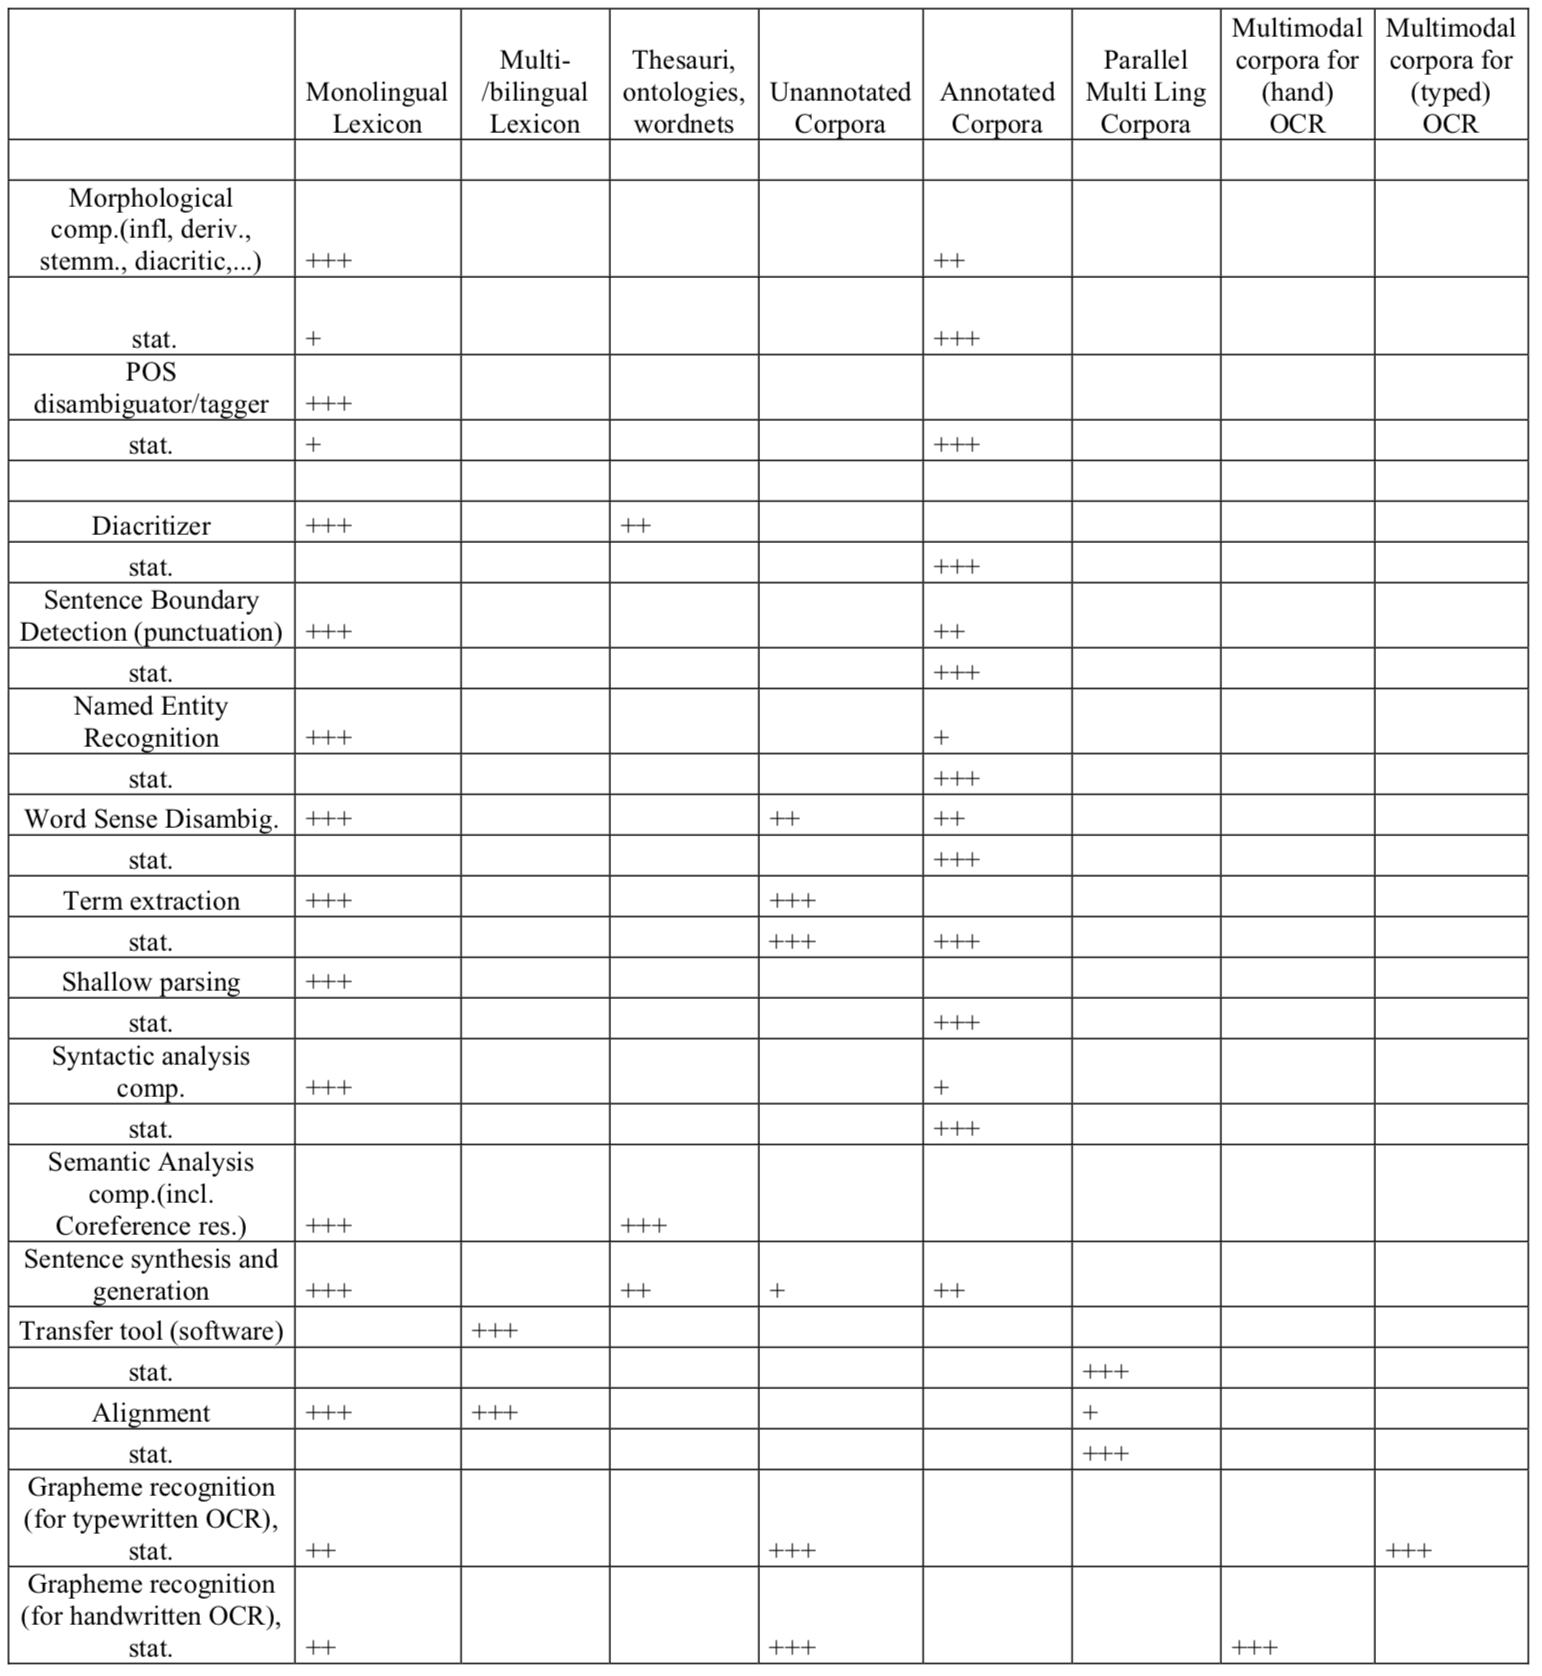
\includegraphics[width=1\textwidth]{img/blark1.png}
 \caption{A BLARK graph for Arabic, with written language applications and corresponding HLT modules, marked with importance \citep[775]{maegaard2006blark}}
 \label{fig:blark1}
\end{figure}

\begin{figure}
 \centering
 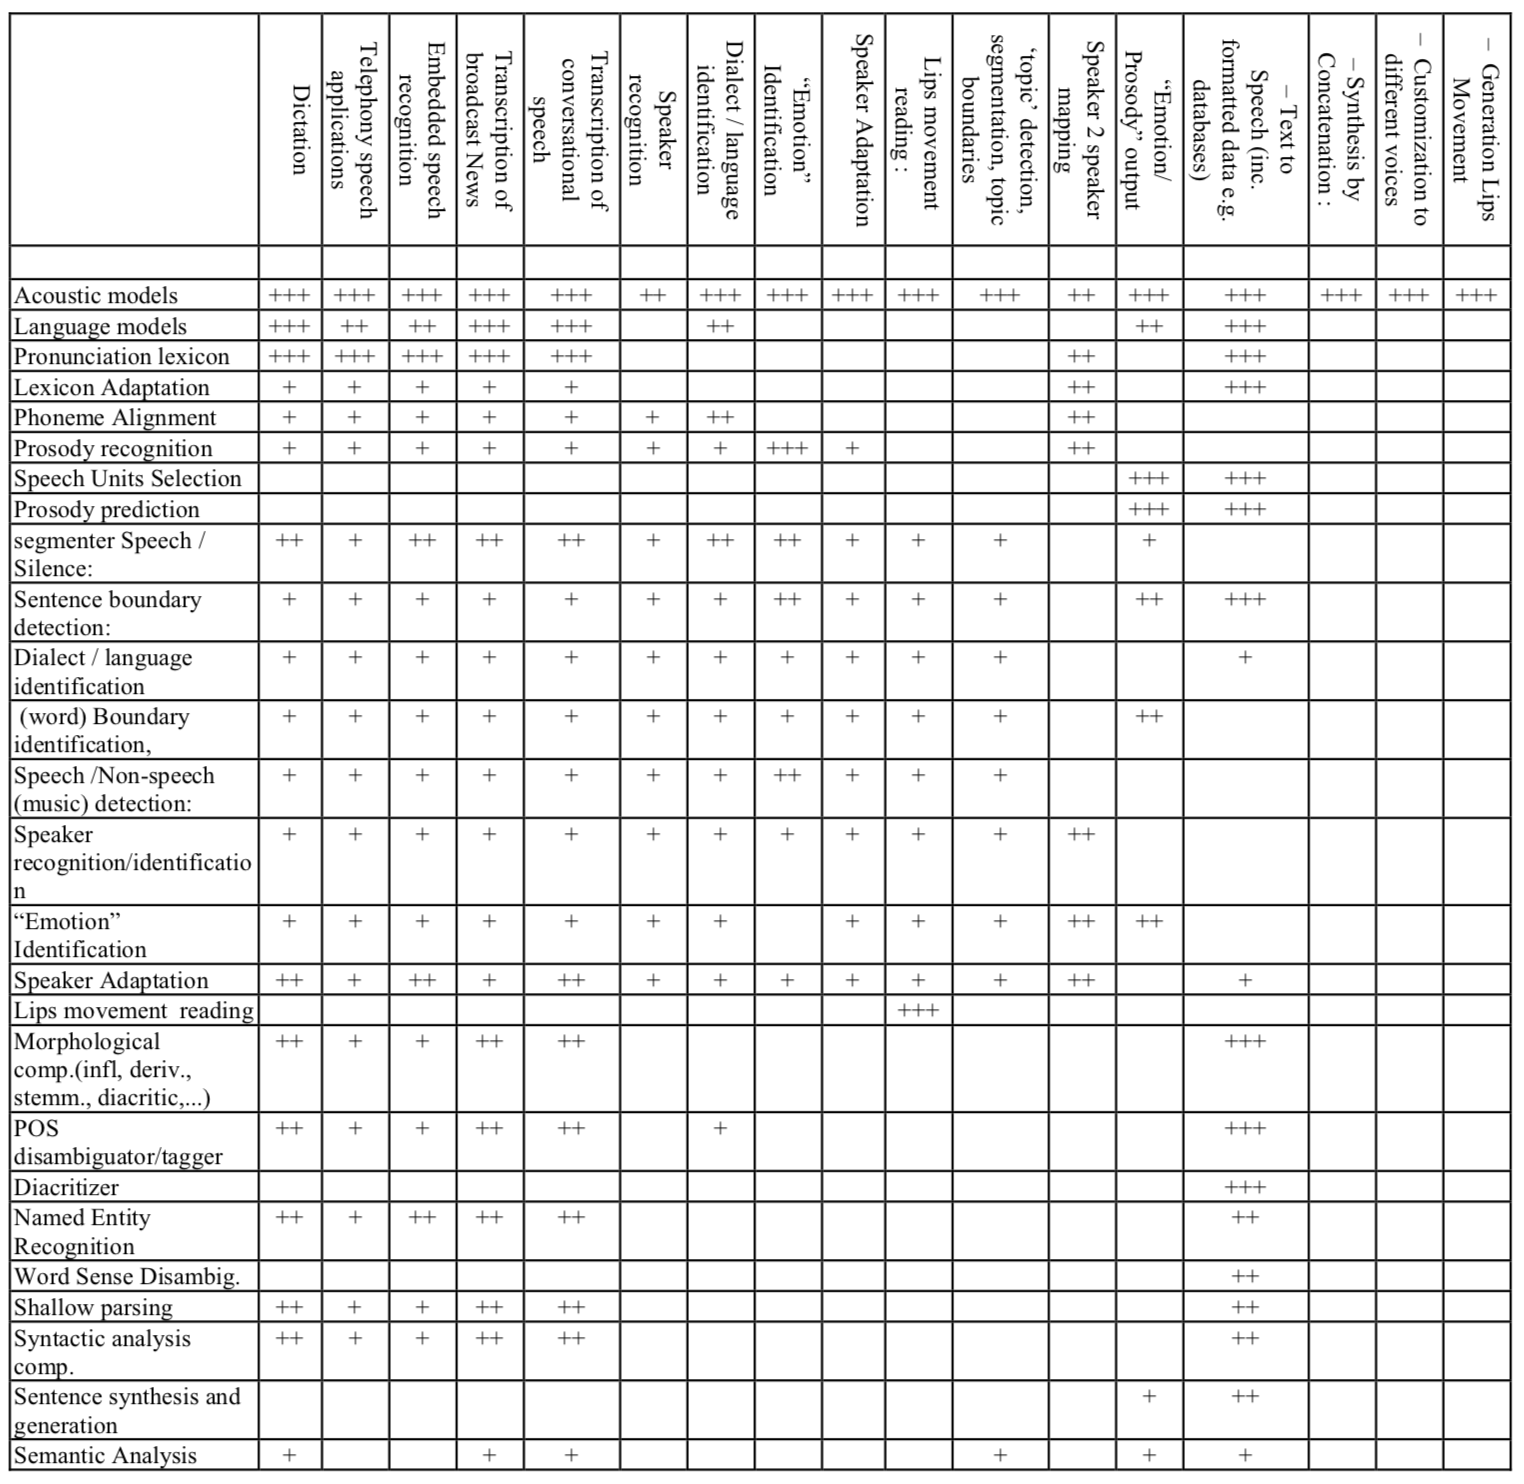
\includegraphics[width=1\textwidth]{img/blark2.png}
 \caption{A BLARK graph for Arabic, with speech language applications and corresponding HLT modules, marked with importance \citep[776]{maegaard2006blark}}
 \label{fig:blark2}
\end{figure}

The BLARK process - auditing a language, using a grid to identify what corpus and resource needs are necessary for language resources - has now been applied to Swedish \citep{elenius2008language} and Bulgarian \citep{simov2004language}, and numerous South African languages \citep{grover2011south}, among others.

Unfortunately, BLARK (or ELARK, purportedly a more sophisticated version of BLARK for industry described in \citet{mapelli2003report}, according to \citep{grover2011south}) is a large grid, and may not work for languages without extensive funding models or support. For this, there is a smaller BLARK version, the BLARKette, which should work for low resource languages (although how a smaller version of a minimal set could be provided usefully is not clear).

\begin{quote}
In order to accommodate this problem we have proposed the definition of a scaled down, entry-level version of the BLARK, targeting exclusively the research and (especially) the education community. It should be light and compact, not too demanding in terms of hard and software requirements, cheap, free from IPR issues, and ideally small enough to fit on a CD or DVD. We expect to release a first document, with tentative summary specifications, towards the end of 2006. Check the ELSNET site for news. \citep{krauwer2006strengthening}
\end{quote}

The model of transportation for this - a CD, instead of a downloadable resource - shows that the concept has not aged well. There is a also surfeit of references of BLARK or BLARKette in the past decade in the literature - \citet{krauwer1998elsnet} only has 31 references on Google Scholar (an imperfect but effective metric).\footnote{\href{https://scholar.google.ca/scholar?cites=5069727220703395724}{https://scholar.google.ca/scholar?cites=5069727220703395724}} What happened? It is most likely (in my opinion) that building a BLARK for a language is too complex for language groups to perform, and lacks proper incentives. It requires an authoritative and intimate knowledge of a language's space by many researchers, all of whom must come together to identify gaps, often from proprietary institutions. This is a difficult task.

But this effort, in some sense, has expanded into LRE (Language Resources and Evaluation) maps within Europe. As described in \citet{calzolari2010lrec, del2014lremap, mariani2015language, del2015visualising}, the Language Resources and Computation (LREC) conference organisers began asking conference participants who had submitted papers to fill out basic language resource grids when submitting papers. This effort was extended to ten different computational linguistics conferences, covering most large European languages and four regional Spanish languages. This data has been collected into matrices and a database that reflects language resources for a variety of languages. To date, this is the most comprehensive review of NLP per language that I'm aware of, with 4395 entries - however, it's worth noting that it is limited in scope. The 133 less-common languages represented in the LRE map represent only 414 entries. An example of the matrix for the high resource languages can be seen in Figure~\ref{fig:lre}, which is a map of resources for various languages, cut off with a lower bound of 50 citations per resource type.

\begin{figure}
 \centering
 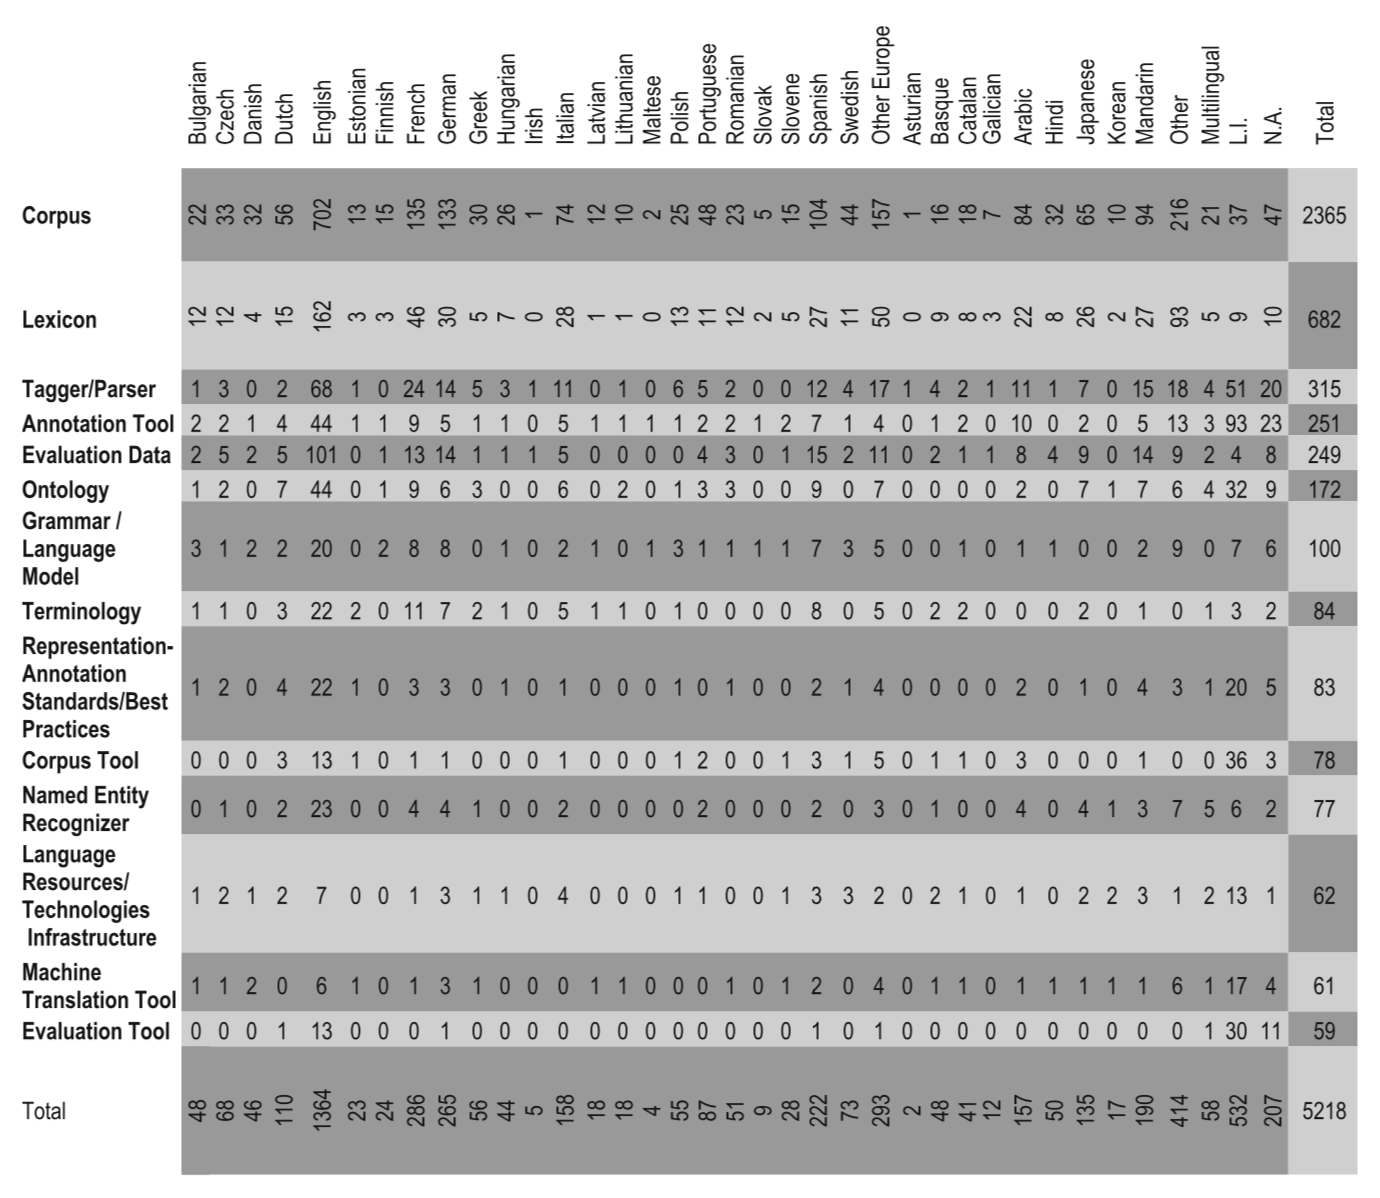
\includegraphics[width=1\textwidth]{img/lre.png}
 \caption{LRE maps for high resource languages \citep[460]{mariani2015language}}
 \label{fig:lre}
\end{figure}

Several authors working on LRE maps are also authors of the \citet{soria2017digital} paper; extending the LRE maps for low resource languages, and then intensifying efforts to develop low-hanging fruit for low resource languages is a logical next step for this research. The focus on European languages is expected; this may stem from the fact that LREC, the main conference series from which LRE data was drawn, is run by the European Language Research Association (ELRA). This fragmentation of the field is unsurprising, and happens in the reverse, as well: for example, \citet{paricio2010new} cites a framework for upgrading low resource languages which is explained in a research paper written in Spanish, and, anecdotally, around half of the papers presented at the Ryukyuan Heritage Language Society's conference in Tokyo in 2012 (which I attended) were presented in Japanese. This is not to say that fragmentation and diversity of linguistics in academia is something to be avoided, but rather that it is a hurdle to be noted and worked with to avoid repeated work and splintered efforts.

%\subsection{The current state of language diversity}
%
%In this section, I am going to briefly go into detail about what diversity means for linguistics. This will be useful later for explaining how related languages can be used to bootstrap work in similar languages. For instance, Irish spell-checkers and constitutional corpora from the EU can be used by Scottish Gaelic speakers with some tweaks in order to further improve their own systems.
%

\subsection{Who makes resources for languages?}
Another hurdle which was briefly alluded to earlier was the plethora of large organisations, databases, or projects dedicated to cataloguing low resource languages. Each of these has differences in scope, funding, and incentives. However, large organisations are not the only groups working on language development, digital ascent, language revitalisation, or any other shared focus that relates to low resource languages.

As \citet{hammarstrom2015unesco} points out, "language documentation and description is an extremely decentralized activity, carried out by missionaries, anthropologists, travellers, naturalists, amateurs, colonial officials, ethnographers and not least linguists over several hundred years." Language communities, amateur and professional linguists, educators, and language policy setters are most often involved in standardising a language and helping to document and revitalise low resource languages. Digitally, amateur computational linguists, and coders who are first language speakers of their own language are often the first to work on translating or migrating resources; this group is also often the first to set up Wikipedias in a local language (although this often leads to enthusiastic loners working outside of the main language communities) \citet{soria2017digital}. Beyond these groups, universities, local governments and businesses can also often develop language resources for low resource languages, as was the case with \citet{rognvaldsson2009icelandic}. After these groups, large grant-driven institutions such as CLARIN or the NSF fund a large portion of language development, along with industry giants such as Google or Xerox, and large military research arms such as DARPA.

Unfortunately, the lion's share of the overall funding for language development goes to languages which are already resourced.

\begin{quote}
Over the years the EU has invested massively in the development of language and speech technology, and many dedicated R\&D programmes have had a significant impact on its advancement, including applications oriented towards solving the multilinguality problem... Unfortunately the strong industrial bias of recent EU programmes has led to a situation where the major part of the funding for language and speech technology goes to the major languages. This is not surprising, as industrial players will prefer to invest in the development and deployment of technologies for larger markets. As a consequence there has been only marginal support for the development of language and speech technology for the language communities that do not constitute profitable markets. As the development cost of such technologies is independent of the number of speakers of a language ("all languages are equally difficult") this has created a very unbalanced situation. \citep{krauwer2006strengthening}
\end{quote}

Or:

\begin{quote}
Were it not for the special attention DARPA, one of the main sponsors of machine translation, devoted to Haitian Creole, it is dubious we would have any MT aimed at this language. There is no reason whatsoever to suppose the Haitian government would have, or even could have, sponsored a similar effort \citep{spice}. \citep[9]{kornai2013digital}
\end{quote}

Another good example of where funding and incentives for language development can be controversial would be Ethnologue, which rate limits and has a paywall guarding usage of their database, even though they are widely recognised as one of the best informed databases for language data. SIL International also gatekeeps the standard ISO 639-3, which is the most widely used language code. By having a paywall on their data, they exclude the general public from having control of codes for their own languages. SIL has also come under criticism for their Christian missionary work, as it can be viewed as complicit in culture change, and by extrapolation, ethnocide \citep{dobrin2009sil, dobrin2009practical, everett2009don}. This is just one example - and most likely one of the most extreme, not counting military work on languages used by insurgents in wars - of how organisations working on language resources may influence the work itself.

The funding of language resource development matters, because the way that the language community approaches language development affects the chance of survival for the language. This is one of the reasons that \citet{grenoble2016response} pointed out that "language vitality" is a more politically correct term to use than "language endangerment", as it takes the focus away from loss and focuses attention on language ascent. Another reason that language funding matters is because the major players with funding will generally be able to out manoeuvre smaller groups with different resources. This can enforce language shift, and can render resources created by individual developers moot. For instance, the secwepemc-facebook\footnote{\href{https://github.com/kscanne/secwepemc-facebook}{https://github.com/kscanne/secwepemc-facebook}} tool developed to automatically translate Facebook into low resource languages, created by the developer Neskie Manuel for his native Secwepemcts\'in, is no longer an active project and has not been updated, rendering it obsolete with Facebook UI changes, while automatic translation is provided for high resource languages natively by Facebook. Scannell, who helped port the secwepemc-facebook tool to Greasemonkey, was one of the authors of \citet{streiter2006implementing}, which suggested that developers for low resource languages use open source software pools in order to pool resources to enable them to overcome this - among other - issues facing low resource languages in particular.

As in Section~\ref{subsubsec:response}, covering all of the potential issues with funding and the politics of language development is well beyond the scope of this paper. However, focusing on how open source can help low resource languages is not. But first; what do I mean by "open source"?

% Here, I will explain briefly who makes language resources for these languages. I'll explain what I see as the main groups doing this work: professional translators, educators, missionaries (of multiple faiths, but mostly Christian), academics and native technologists. I'll explain each stakeholder and their canonical perspectives.

% Alexis: what do you mean by "their canonical perspectives"? will this section address creation of digital resources only, or all resources? for that matter, what counts as a digital resource? does a collection of pdf scans of old books count? how about a pdf version of a text collection? etc....
% I don't immediately see how this fits into the rest of the thesis. also look at relevant publications from Jeff Good - one in particular on the ecology of language documentation: http://www.acsu.buffalo.edu/~jcgood/publications.html


%\subsection{Language research funding}
%
%Here, I'll go into more depth about funding, as we've outlined who works on LRLs and who would fund research, and why. This will further inform the basis for the work of the previous section. I'll talk about DARPA MT funding in the 20th century, as well as other efforts such as CLARIN.



% IARPA and DARPA both are involved with low resource languages and both of them may have their own institutional values that are probably at ends with independent researchers, commercial consumers, and language communities. Does working on sparse data openly bring along with it ethical or moral concerns; if so, how can these be adequately explained, breached, and talked about? How can they be worked around or be part of the conversation? Note that DARPA and the like also use humanitarian reasons as their primary stated aim for work on sparse languages, which may be contrary to their military needs. There is already an extensive literature on moral uses of data -- I could summarize that, and apply it specifically to low resource languages, which is something I do not think has yet been published.

% Darpa: http://www.darpa.mil/program/low-resource-languages-for-emergent-incidents
% IARPA: http://www.iarpa.gov/index.php/research-programs/babel

% - Institutional bottleneck
% - Linguistic colonialism
% - Ethical and moral concerns for military usage
% - Ethical and moral concerns for big business usage



%% TODO include this, formerly in introduction

%Incidentally, there is something to be said for spoken language corpora, which may be more prevalent in some cases than written resources (especially in a region with a history of radio transmissions in the local language, for instance). However, the direct use of spoken language corpora for building language resources is limited and generally requires more processing and development time (not to mention storage), compared to cheap, written data.
% Alexis: also what about spoken language corpora? e.g. work by Oliver Adams & colleagues inducing linguistic information from spoken data, skipping the usual transcription set. I'm not saying you need to also deal with spoken language data, but it does need to be acknowledged